\documentclass[10pt]{article}
\usepackage[utf8]{inputenc}

\usepackage{fullpage}
\usepackage{amsmath,amssymb, amsfonts,amsthm, enumerate}
\usepackage{mathbbol}
\usepackage{graphicx}

\usepackage{booktabs}  % nice looking tables
\usepackage{numprint}
\npdecimalsign{.}
\nprounddigits{2}

% these are compressed lists to help fit into a 1 page limit
\newenvironment{enumerate*}%
  {\vspace{-2ex} \begin{enumerate} %
     \setlength{\itemsep}{-1ex} \setlength{\parsep}{0pt}}%
  {\end{enumerate}}
 
\newenvironment{itemize*}%
  {\vspace{-2ex} \begin{itemize} %
     \setlength{\itemsep}{-1ex} \setlength{\parsep}{0pt}}%
  {\end{itemize}}
 
\newenvironment{description*}%
  {\vspace{-2ex} \begin{description} %
     \setlength{\itemsep}{-1ex} \setlength{\parsep}{0pt}}%
  {\end{description}}
  
\title{Stat 221 Problem Set 5}
\author{Albert Young and Marco Gentili}
\date{18 November 2014}

\begin{document}

\maketitle

\section*{Question 1.1}
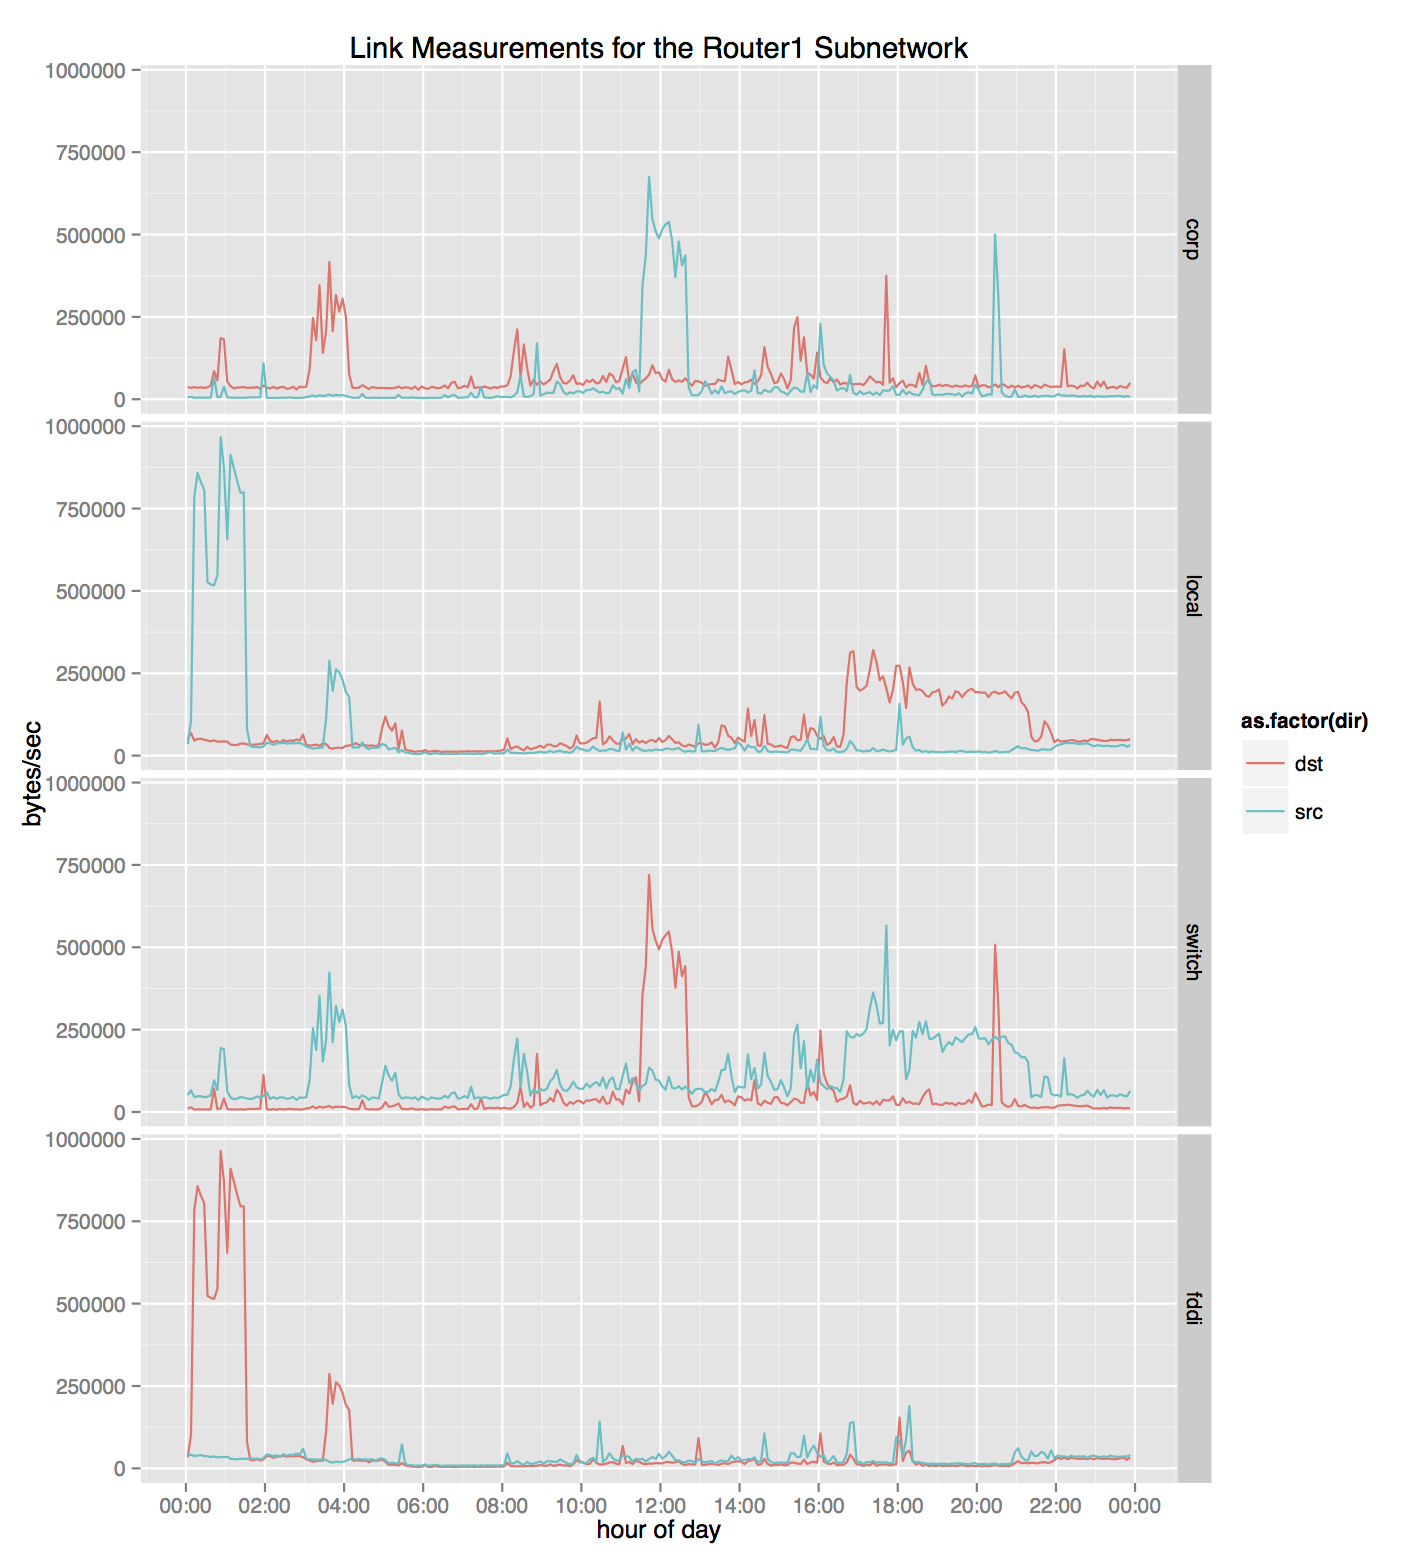
\includegraphics[scale=0.75]{YoungGentili_fig2.png}\\
\section*{Question 1.2}
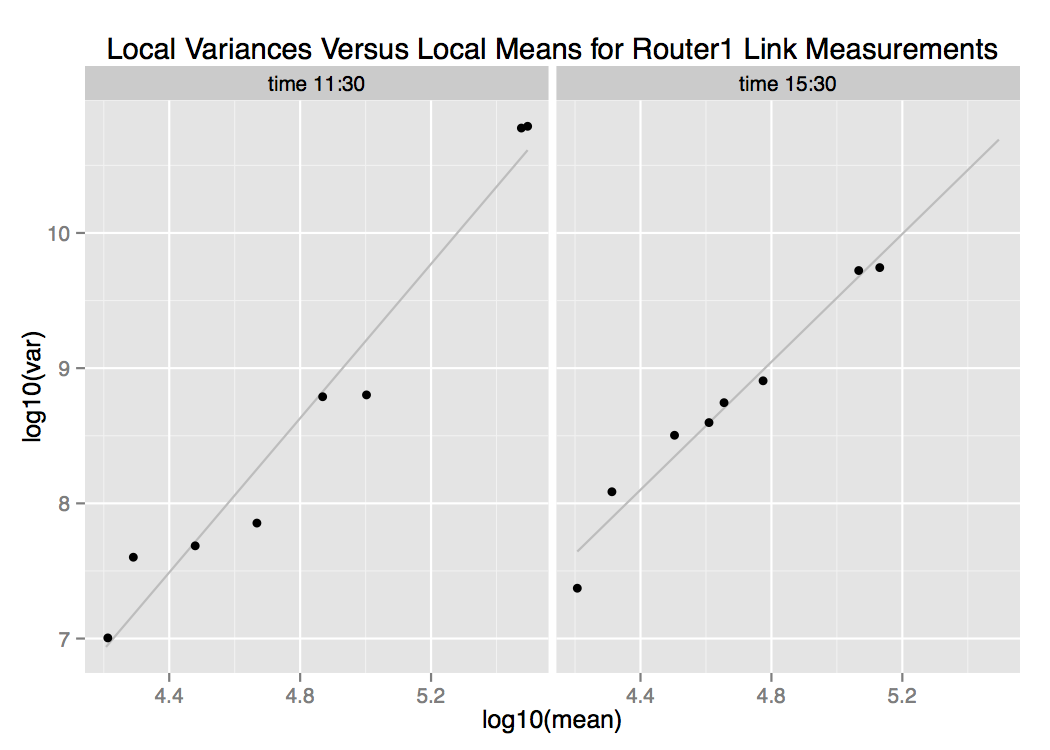
\includegraphics[scale=0.8]{YoungGentili_fig4_1router.png}\\
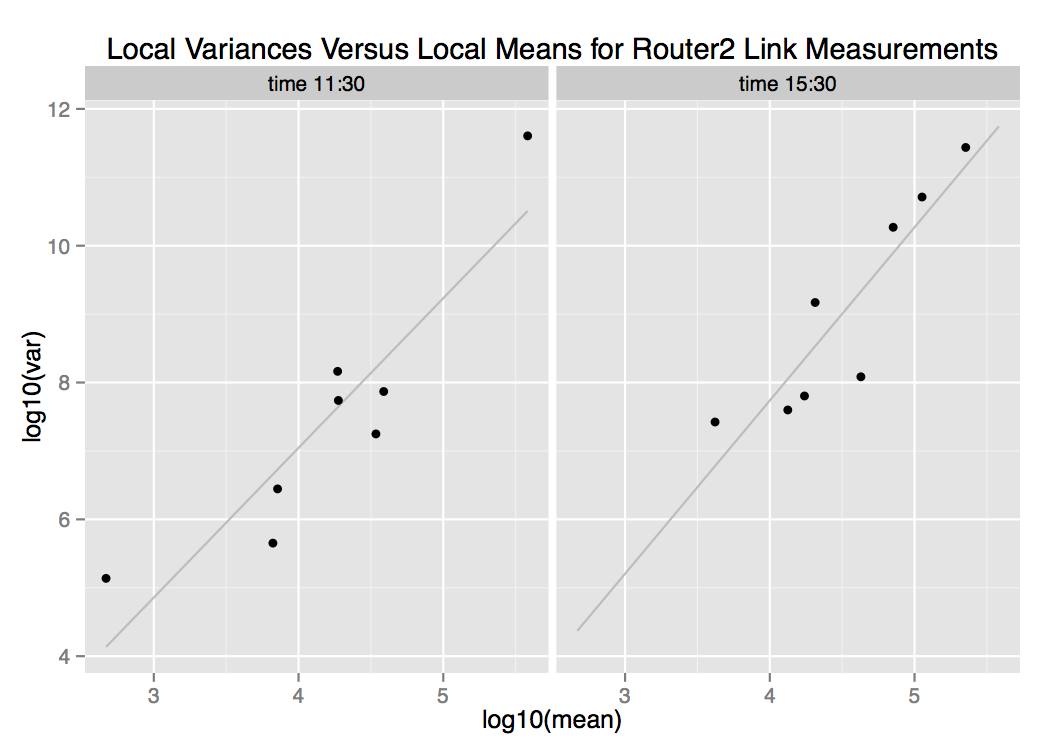
\includegraphics[scale=0.8]{YoungGentili_fig4_2router.png}\\
\section*{Question 1.3}
The unobserved OD byte counts, $\mathbf{x}_t$ at time $t$ are modeled as a vector of independent normal random variables:
\begin{align}
\mathbf{x}_t \sim N(\mathbf{\lambda}, \mathbf{\Sigma})
\end{align}
The complete data log-likelihood is:
\begin{align}
l(\mathbf{\theta}|\mathbf{X})=-\dfrac{T}{2}\log{|\mathbf{\Sigma}|}-\dfrac{1}{2}\sum_{t=1}^T (\mathbf{x}_t - \lambda)'\mathbf{\Sigma}^{-1}(\mathbf{x}_t-\mathbf{\lambda})
\end{align}
The EM conditional expectation function $Q$ is
\begin{align}
Q(\mathbf{\theta}, \mathbf{\theta}^{(k)}) &= \mathbf{E}(l(\mathbf{\theta}|\mathbf{X})|\mathbf{Y}, \mathbf{\theta}^{(k)})\\
&= \mathbf{E}\left[-\dfrac{T}{2}\log{|\mathbf{\Sigma}|} - \dfrac{1}{2}\sum_{t=1}^T (\mathbf{x}_t - \lambda)'\mathbf{\Sigma}^{-1}(\mathbf{x}_t-\mathbf{\lambda})\right]\\
&= -\dfrac{T}{2}\log{|\mathbf{\Sigma}|} - \dfrac{1}{2}\sum_{t=1}^T\mathbf{E}\left[ (\mathbf{x}_t - \lambda)'\mathbf{\Sigma}^{-1}(\mathbf{x}_t-\mathbf{\lambda})\right]
\end{align}
Since $(\mathbf{x}_t - \lambda)'\mathbf{\Sigma}^{-1}(\mathbf{x}_t-\mathbf{\lambda})$ has a quadratic form, we can use the formula for its expectation
% http://en.wikipedia.org/wiki/Quadratic_form_(statistics)
\begin{align}
\mathbf{E}\left[(\mathbf{x}_t - \lambda)'\mathbf{\Sigma}^{-1}(\mathbf{x}_t-\mathbf{\lambda})\right]&=\mathrm{tr}\left(\mathbf{\Sigma}^{-1}\mathrm{Var}(\mathbf{x}_t-\mathbf{\lambda}|\mathbf{y}_t,\mathbf{\theta}^{(k)})\right) + \mathbf{E}(\mathbf{x}_t-\mathbf{\lambda}|\mathbf{y}_t,\mathbf{\theta}^{(k)})'\mathbf{\Sigma}^{-1}\mathbf{E}(\mathbf{x}_t-\mathbf{\lambda}|\mathbf{y}_t,\mathbf{\theta}^{(k)})\\
&=\mathrm{tr}\left(\mathbf{\Sigma}^{-1}\mathrm{Var}(\mathbf{x}_t|\mathbf{y}_t,\mathbf{\theta}^{(k)})\right) +(\mathbf{m}_t^{(k)}-\mathbf{\lambda})'\mathbf{\Sigma}^{-1}(\mathbf{m}_t^{(k)}-\mathbf{\lambda})\\
&=\mathrm{tr}\left(\mathbf{\Sigma}^{-1}\mathbf{R}^{(k)}\right) +(\mathbf{m}_t^{(k)}-\mathbf{\lambda})'\mathbf{\Sigma}^{-1}(\mathbf{m}_t^{(k)}-\mathbf{\lambda})
\end{align}
where
\begin{align}
\mathbf{m}_t^{(k)} &= \mathbf{E}(\mathbf{x}_t|\mathbf{y}_t,\mathbf{\theta}^{(k)})\\
&= \mathbf{\lambda}^{(k)} + \mathbf{\Sigma}^{(k)}\mathbf{A}'(\mathbf{A}\mathbf{\Sigma}^{(k)}\mathbf{A}')^{-1}(\mathbf{y}_t - \mathbf{A}\mathbf{\lambda}^{(k)}),\\
\mathbf{R}^{(k)} &= \mathrm{Var}(\mathbf{x}_t|\mathbf{y}_t,\mathbf{\theta}^{(k)})\\
&= \mathbf{\Sigma}^{(k)} - \mathbf{\Sigma}^{(k)}\mathbf{A}'(\mathbf{A}\mathbf{\Sigma}^{(k)}\mathbf{A}')^{-1}\mathbf{A}\mathbf{\Sigma}^{(k)}
\end{align}
Here we have taken advantage of the conditional distributions of a multivariate normal.\\
% http://stats.stackexchange.com/questions/30588/deriving-the-conditional-distributions-of-a-multivariate-normal-distribution
% http://en.wikipedia.org/wiki/Multivariate_normal_distribution
We can plug (8) back into (5) to obtain eq. 6 in Cao et al. (2000), completing the derivation.
\subsection*{The EM algorithm}
\begin{enumerate}
\item E-step: Calculate $\mathbf{m}_j^{(k)}$ and $\mathbf{R}^{(k)}$. If $k=0$ we must initialize the values.
\item M-step: Maximize $Q(\mathbf{\theta}, \mathbf{\theta}^{(k)})$ with respect to $\mathbf{\theta}$.
\item Repeat steps 1 and 2 until convergence.
\end{enumerate}
\section*{Question 1.4}
To fit the EM algorithm derived for the iid model to the locally iid model, we simply modify the $Q$ function. To estimate the parameters at each time point t, instead of summing over all time points $[1, T]$, we only sum over time points in our window, which are assumed to be iid normal:
\begin{align}
Q(\mathbf{\theta}, \mathbf{\theta}^{(k)})=\mathbf{E}\left[-\dfrac{w}{2}\log{|\mathbf{\Sigma}|} - \dfrac{1}{2}\sum_{j=t-h}^{t+h} (\mathbf{x}_j - \lambda)'\mathbf{\Sigma}^{-1}(\mathbf{x}_j-\mathbf{\lambda})\right]
\end{align}
Initializing $\theta$ to $\vec{0}$ and running EM until an absolute convergence threshold of 1E-4, we successfully replicated Figure 5:\\
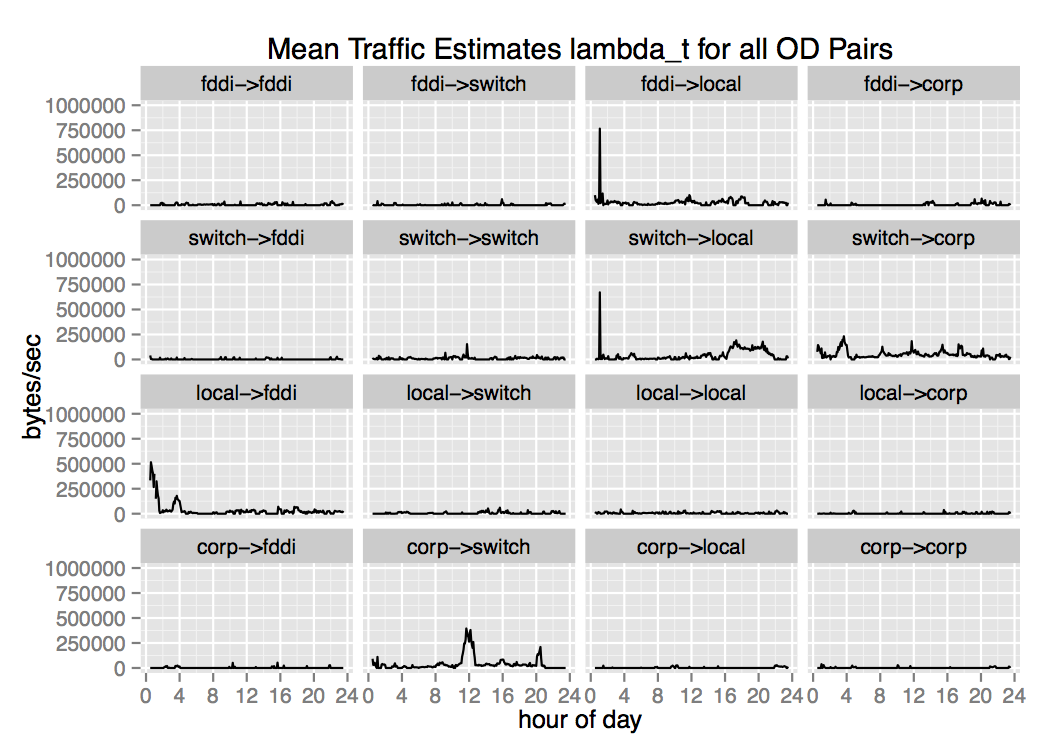
\includegraphics[scale=1]{YoungGentili_fig5.png}\\

\section*{Question 1.5}
In this section, we let $\eta_t = (\log(\lambda_t), \phi(t) )$, and have the update $\eta_t = \eta_{t-1} + v_{t}$, where $v_t \sim N(0, V)$, where $V$ is a fixed variance matrix that we choose beforehand (per suggestions, we set it equal to 5*diag(exp(lambda)) ).\\

We have that $p(\eta_t | \tilde{Y}_{t}) = p(\eta_t | \tilde{Y}_{t-1}, Y_t) \propto p(\eta_t | \tilde{Y}_{t-1})p(Y_t | \eta_t )$, so that $\log p(\eta_t | \tilde{Y}_{t-1}, Y_t) \propto \log p(\eta_t | \tilde{Y}_{t-1}) + \log p(Y_t | \eta_t )$. The first term on the right hand side is the prior and the second is the likelihood.\\

Thus, the process for maximizing our posterior $\log p(\eta_t | \tilde{Y}_{t-1}, Y_t)$ is the same as before except with our additive penalty correction $\log p(\eta_t | \tilde{Y}_{t-1})$.\\

We have that $$p(\eta_t | \tilde{Y}_{t-1}) \propto \int p(\eta_{t-1} | \tilde{Y}_{t-1})p(\eta_t | \eta_{t-1})d \eta_{t-1}$$
If we approximate $p(\eta_{t-1} | \tilde{Y}_{t-1})$ by $N(\hat{\eta}_{t-1}, \hat{\Sigma}_{t-1})$, where $\hat{\eta}_{t-1}$ is the posterior mode and $\hat{\Sigma}_{t-1}$ is the inverse of the curvature of the log posterior density at the mode, then we can approximate $ p(\eta_{t} | \tilde{Y}_{t-1})$ by $N(\hat{\eta}_{t-1}, \hat{\Sigma}_{t-1} + V)$.\\

So now our $Q$ function is the same as that from part 4 except with this added term 
$$-\dfrac{w}{2}\log{|\hat{\Sigma}_{t-1} + V|} - \dfrac{1}{2}(\mathbf{\eta} - \hat{\eta}^{(k)})'\left(\mathbf{\hat{\Sigma}_{t-1} + V}\right)^{-1}(\mathbf{\eta} - \hat{\eta}^{(k)})
$$

Our algorithm is then as described in the paper:
\begin{enumerate}
\item Initialize $t = h + 1, \hat{\eta}_{t-1} = \hat{\eta}_0, \Sigma_{t-1} = \Sigma_0$
\item Set $\hat{\Sigma}_{t | t-1} = \hat{\Sigma}_{t-1} + V$ and $\pi(\eta_t) = p(\eta_t | \tilde{Y}_{t-1}) \sim N(\hat{\eta}_{t-1}, \hat{\Sigma}_{t | t-1})$, which is the prior of $\eta_t$ given observations $\tilde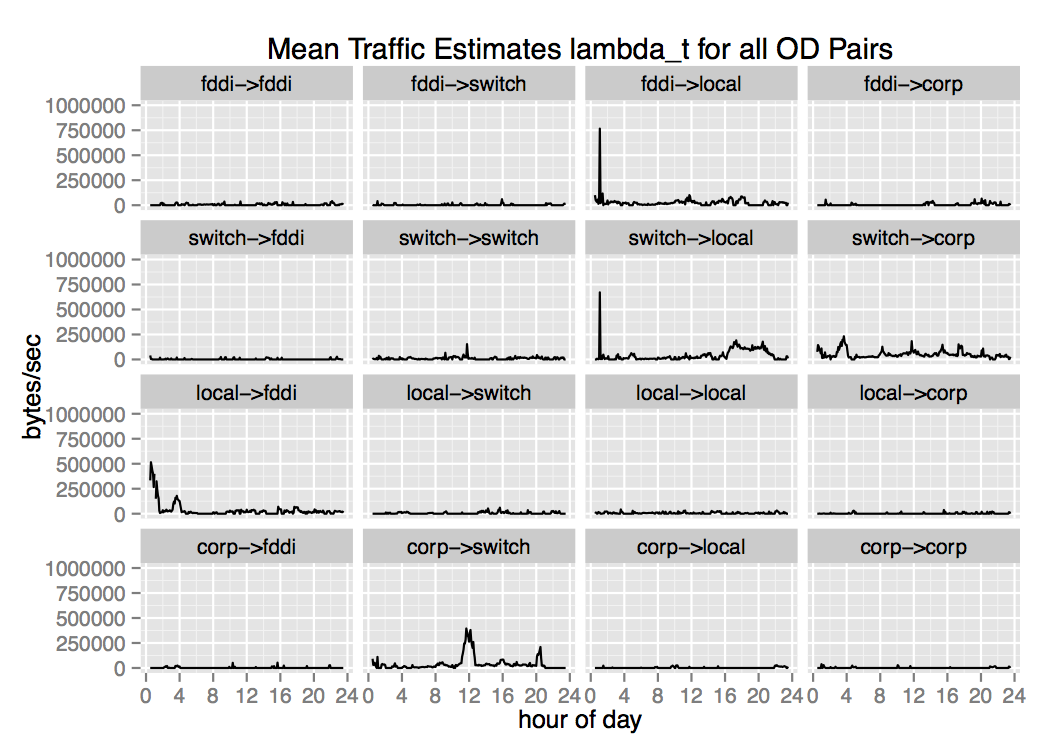
\includegraphics[scale=1]{YoungGentili_fig5.png}\\{Y}_{t-1}$ as described before.
\item Define $g(\eta_t)$ to be $\log \pi(\eta_t) + \log p(Y_t | \eta_t )$. Find the mode $\hat{\eta}_t$ using optim
\item Update $\hat{\Sigma}_t = \ddot{g}(\hat{\eta}_t)^{-1}$, where $\ddot{g}(\eta_t) = -\hat{\Sigma}_{t | t-1}^{-1} + \dfrac{\partial^2 \log p}{\partial \eta_t^2}$
\end{enumerate}
\section*{Question 1.6}
Though evidence of smoothing is shown, we had some issues reproducing Figure 6, in particular evaluating the Hessian matrix.\\
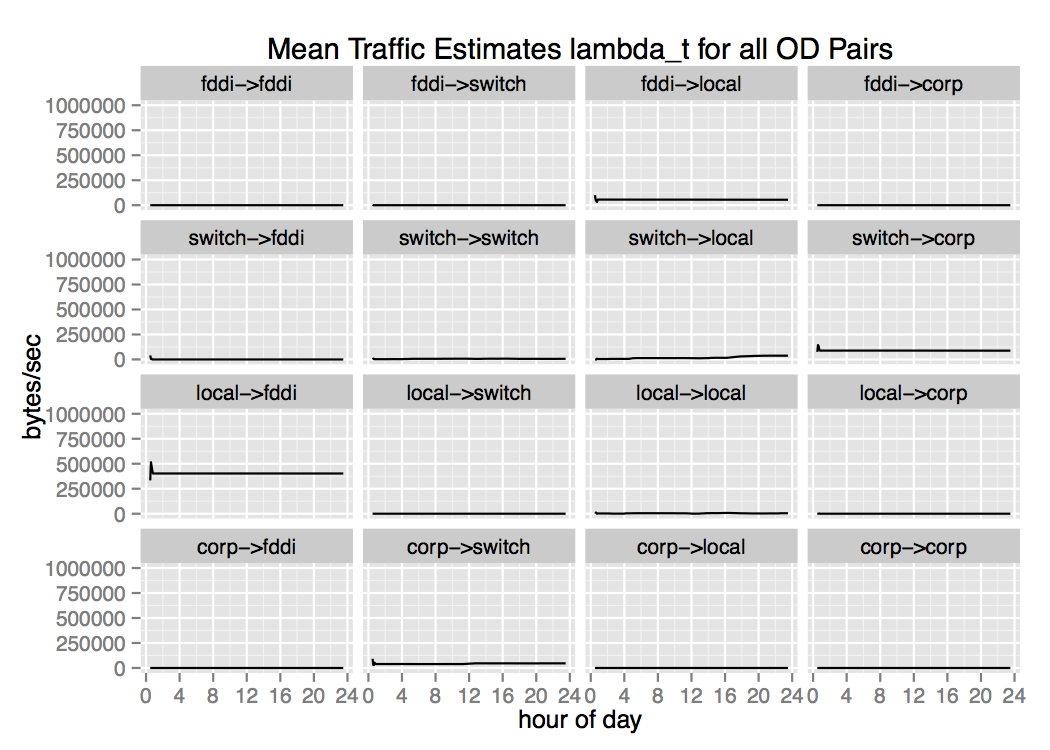
\includegraphics[scale=1]{YoungGentili_fig6_1router.png}\\

\section*{Question 1.8}
The method of Cao et al is more adaptive than that of Tebaldi and West. More specifically, it allows for continuous measurements of data over time, and changes in the parameters of the model accordingly. Tebaldi and West instead fix their model for a certain time interval. Networks are dynamic (there may be more traffic during morning hours, after people wake up, and a lull after 5pm, when people leave work, for instance), so we except that a fixed model will not be able to capture all the nuances of time-varying traffic.\\

Tebaldi and West also assume that the network traffic is iid Poisson distributed, while Cao et al say that network traffic can be approximated by iid normals. Cao et al claim that such an approximation is valid given the high speed of today's networks and the use of 5 minute intervals, which makes the discreteness of byte counts negligible. Furthermore, by introducing a $\phi$ parameter, Cao and Yu are able to accommodate a change in units of traffic measurement, so their model is scale-invariant while that of Tebaldi is not. Another benefit of using iid normals rather than iid poissons is the computational efficiency of the former and the computational complexity of the latter. With the iid normal assumption, Cao et al are able to derive equations that allow for use of the Expectation Maximization algorithm to compute the optimal $x$ vector. Tebaldi and West instead used MCMC to sample from the posterior distribution.\\

Cao et al's model also uses a power relation, which is an extension to the Poisson model that allows for overdispersion and a superlinear increase in the variance with the mean, once again making their model more powerful than that of Tebaldi and West.
\section*{Question 1.9}
Below is the locally iid model fit to the link loads of router 2:\\
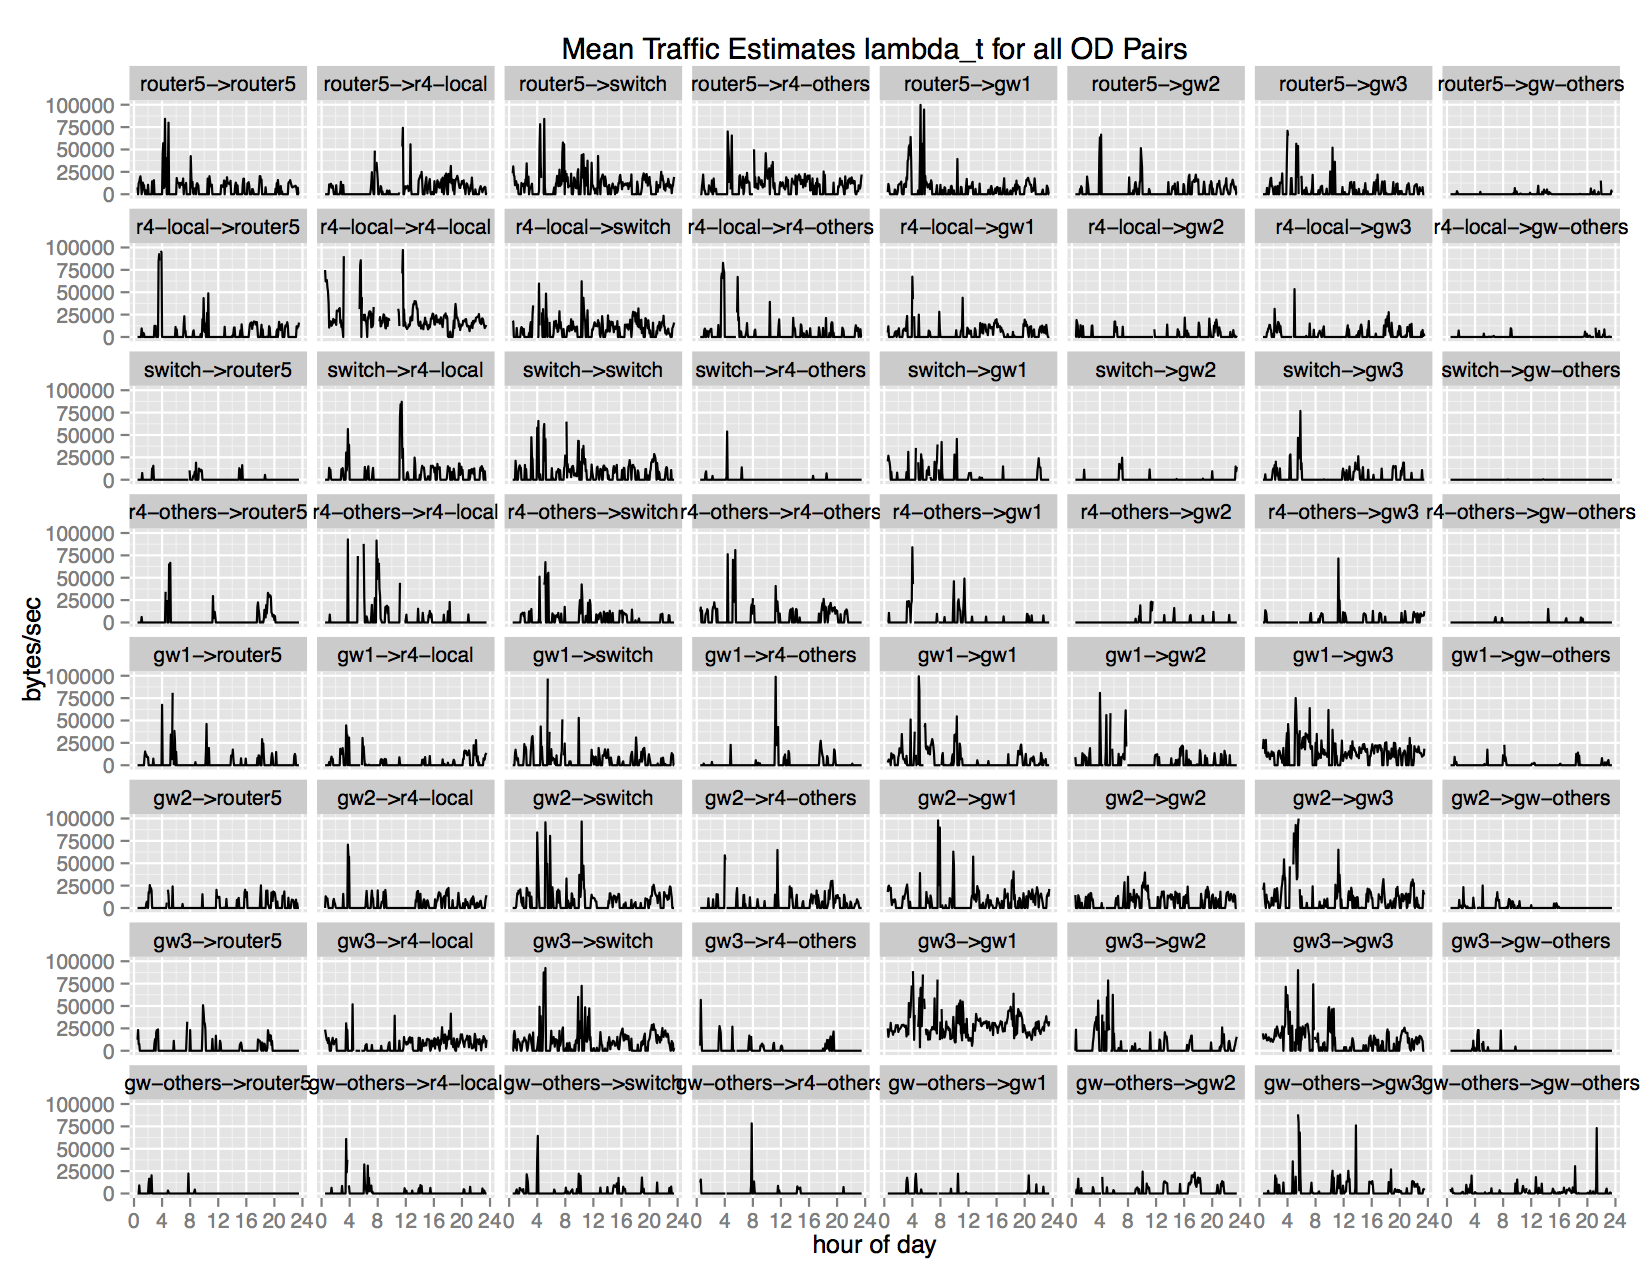
\includegraphics[scale=.6]{YoungGentili_fig9.png}\\
\end{document}
